\newpage
\setcounter{section}{0}
\renewcommand{\thesection}{\arabic{section}}

\begin{center}
    \Huge
    \textbf{Modul 5}
    
    Implementasi dan Konfigurasi IP Version 6

\end{center}


\section{pendahuluan}

Semakin berkembangnya teknologi, maka semakin banyak alokasi alamat jaringan yang diperlukan. Maka dari itu dikembangkanlah Internet Protocol Address v6 (IPV6). Internet Protocol Address v6 (IPv6) adalah standar protokol yang digunakan untuk mengidentifikasi dan mengarahkan alamat jaringan dalam jaringan komputer. Dibandingkan dengan pendahulunya, IPv4, IPv6 memiliki format alamat yang lebih panjang dengan 128 bit, yang memungkinkan jumlah alamat yang jauh lebih besar, sehingga dapat mengatasi kekurangan alamat IPv4 yang semakin berkurang. IPv6 juga mendukung fitur-fitur tambahan, termasuk pemantauan aliran lalu lintas, keamanan yang ditingkatkan, dan kualitas layanan yang lebih baik, menjadikannya solusi jangka panjang untuk pertumbuhan Internet yang pesat dan kebutuhan alamat yang terus berkembang.

\section{Tujuan Praktikum}

\begin{enumerate}
    \item Mengetahui bagaimana konfigurasi static routing menggunakan IPV6
    \item Mengimplementasikan konfigurasi IPV6 pada perangkat mikrotik
\end{enumerate}

\section{Alat dan Bahan}

berikut adalah alat dan bahan yang digunakan:


\begin{enumerate}
    \item 2 Router
    \item 3 Kabel LAN
    \item 2 Laptop
    \item Koneksi Internet
\end{enumerate}

\section{Topologi}

berikut adalah topologi yang digunakan :

\begin{center}
    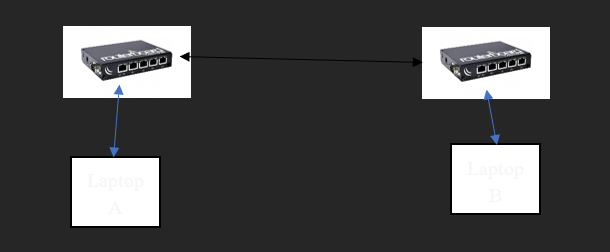
\includegraphics[width=0.7\textwidth]{image/P5/Topologi.png}    
    
    figure.1 Topologi
\end{center}


\section{Langkah Percobaan}
\begin{enumerate}
    \item Persiapan Awal
    
    \begin{enumerate}
        \item Sambungkan PC dan router mikrotik sesuai dengan topologi
        \item Matikan firewall di laptop
        \item Masuk ke aplikasi Winbox
        \item Pada bagian Neighbour, check apakah ada IP 0000 identity mikrotik
        \item Reset mikrotik ke 0000
        \item Lalu tekan connect
    
        \begin{center}
            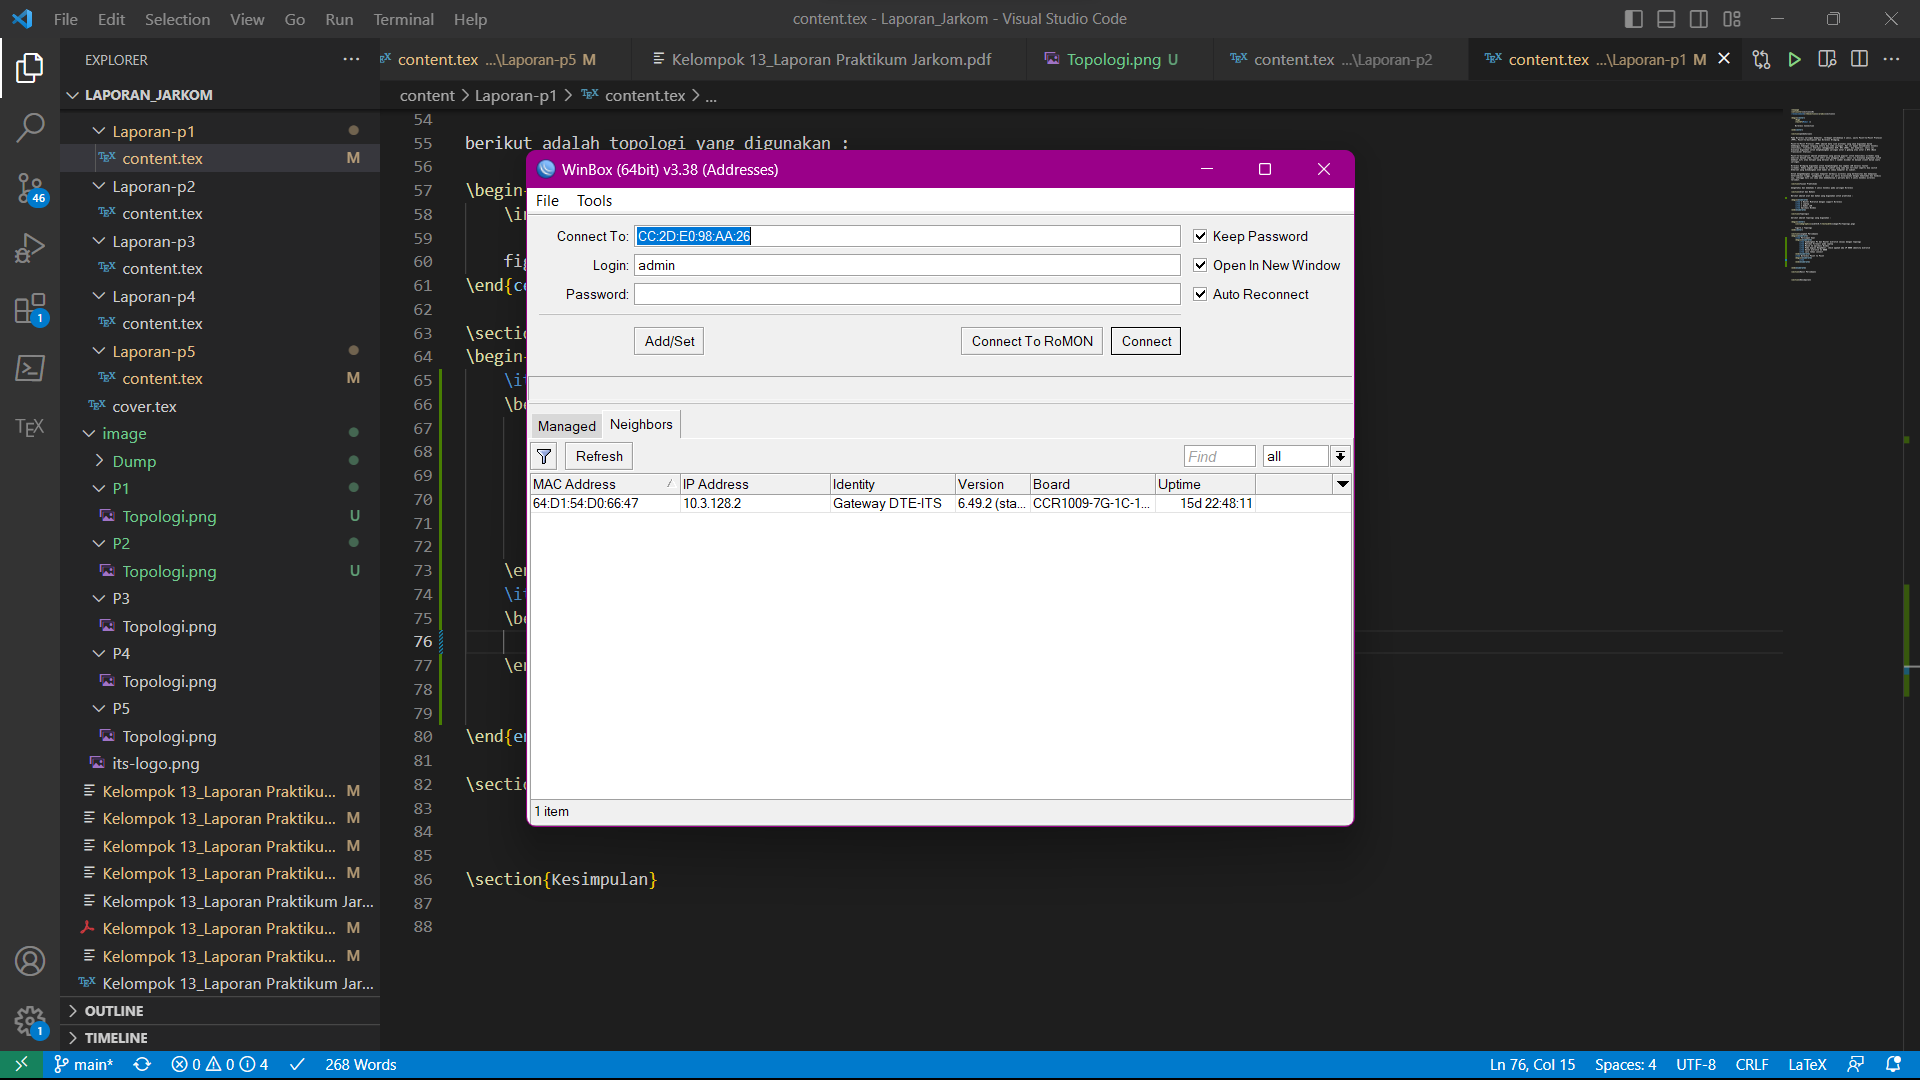
\includegraphics[width=0.7\textwidth]{image/Winbox-interface.png}    
        
            figure.2 WinBox interface
        \end{center}

        \item Aktifkan IPv6 pada kedua router, pilih menu System \texttt{\text>} Packages \texttt{\text>} ipv6 [Enable]
        \item Kemudian reboot router, melalui System \texttt{\text>} Reboot
        \item Pada bagian Neighbour, check apakah ada IP Address versi 6
        \item Lalu tekan connect
        \item Lakukan konfigurasi DHCP agar dapat terhubung dengan ISP, pilih menu IP \texttt{\text>} DHCP Client \texttt{\text>} (+) \texttt{\text>} Interface : ether 1 (yang terhubung pada ISP)
        \item Kemudian secara otomatis akan didapatkan IP dari ISP
    
        \begin{center}
            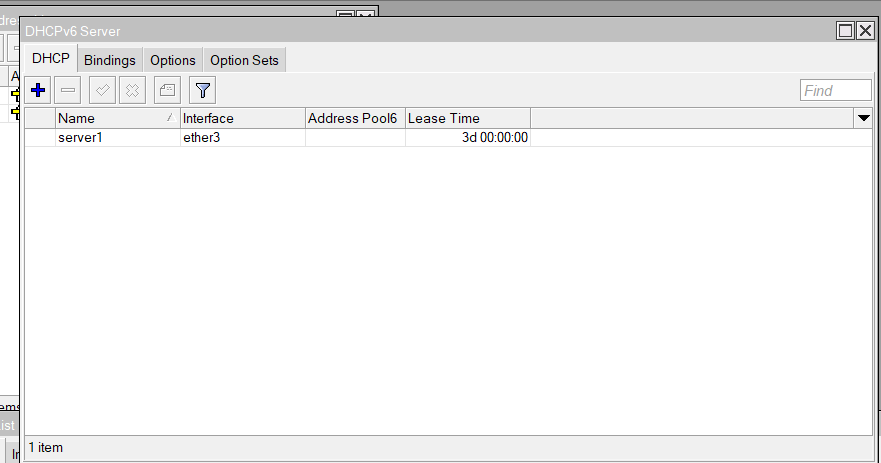
\includegraphics[width=0.7\textwidth]{image/P5/dhcpclient.png}    
        
            figure.3 DHCP Client
        \end{center}
    \end{enumerate}
    
    \item Static v6 Routing
    
    \begin{enumerate}
        \item Konfigurasi IPv6 pada kedua router, pilih menu IPv6 \texttt{\text>} Addresses \texttt{\text>} (+) \texttt{\text>} Address : (IP address versi 6 pada router) , Interface : (Interface yang tersambung ke laptop) , Advertise [Check]
    
        \begin{center}
            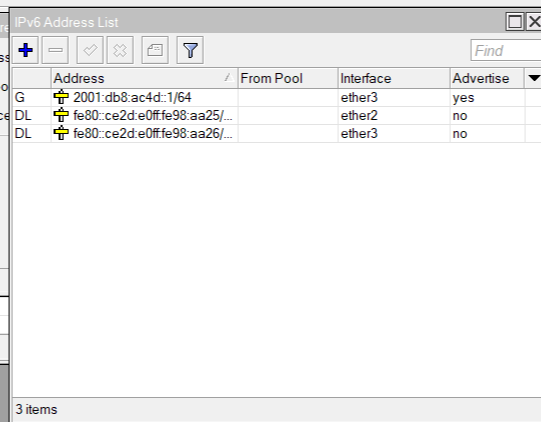
\includegraphics[width=0.7\textwidth]{image/P5/static/static-addresslist.png}    
            
            figure.4 Address List
        \end{center}
    
        \item Selanjutnya lakukan static routing pada masing-masing router (sama seperti melaku\\kan routing IP versi 4), pilih menu IPv6 \texttt{\text>} Routes \texttt{\text>} (+) \texttt{\text>} Dst. Address : (IP versi 6 jaringan lawan) , Gateway : (gunakan link local IP address yang menghubungkan antara kedua router)
        
        \begin{center}
            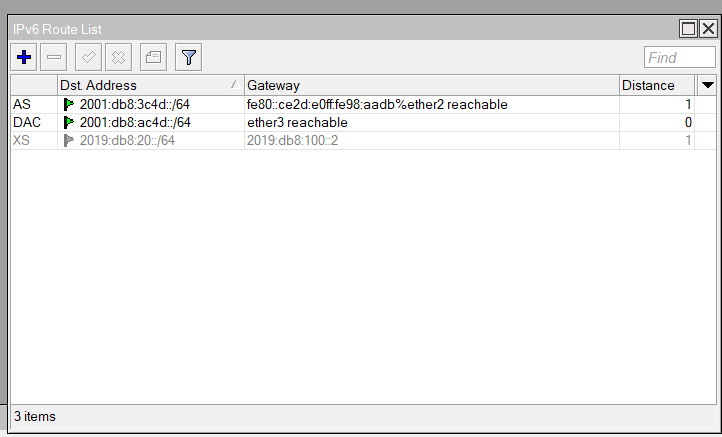
\includegraphics[width=0.7\textwidth]{image/P5/static/static-routing.png}    
            
            figure.5 Static v6 Routing
        \end{center}
    
        \item Setelah itu uji koneksi antara kedua jaringan dengan melakukan test ping dari router (sama seperti melakukan test ping pada IP versi 4)
    \end{enumerate}

    \item Dynamic v6 Routing 
    \begin{enumerate}
        \item Konfigurasi IPv6 pada kedua router, pilih menu IPv6 \texttt{\text>} Addresses \texttt{\text>} (+) \texttt{\text>} Address : (IP address versi 6 pada router) , Interface : (Interface yang tersambung ke laptop) , Advertise [Check]
    
        \begin{center}
            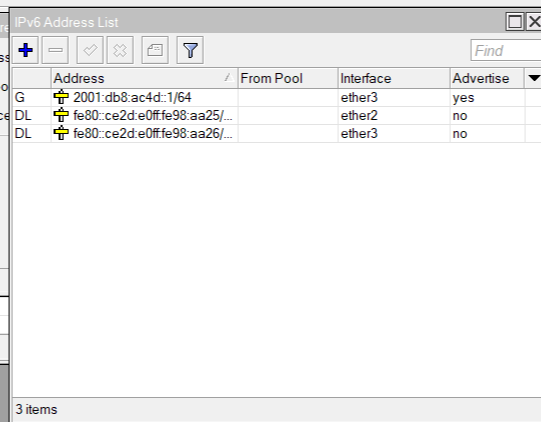
\includegraphics[width=0.7\textwidth]{image/P5/static/static-addresslist.png}    
            
            figure.6 Address List
        \end{center}

        \item selanjutnya lakukan Dynamic Routing dengnan pilih menu Route \texttt{\text>} RIPng \texttt{\text>} (+) \texttt{\text>} interface : (interface yang dipakai)
        
        \begin{center}
            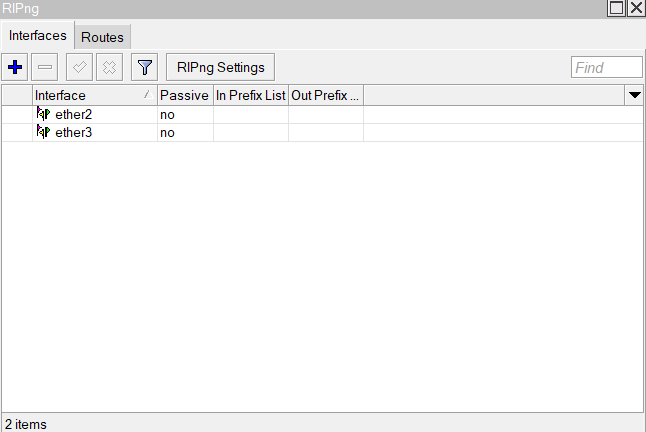
\includegraphics[width=0.7\textwidth]{image/P5/dynamic/dynamic-ripng.png}    
            
            figure.7 RIPng Dynamic v6 Routing
        \end{center}

        \item bila sudah dilakukan dengna benar, maka di routing akan muncul route baru 
        
        \begin{center}
            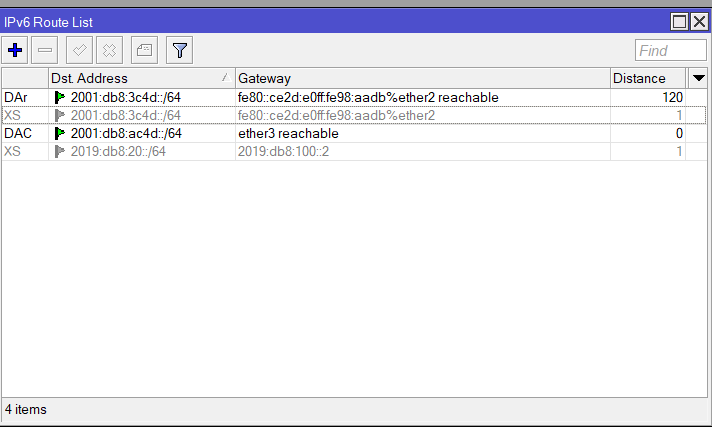
\includegraphics[width=0.7\textwidth]{image/P5/dynamic/dynamic-routing.png}    
            
            figure.8 Dynamic v6 Route
        \end{center}

    \end{enumerate}
    
\end{enumerate}

\section{Hasil Percobaan}

\begin{enumerate}
    \item Static v6 Routing
    
    \begin{center}
        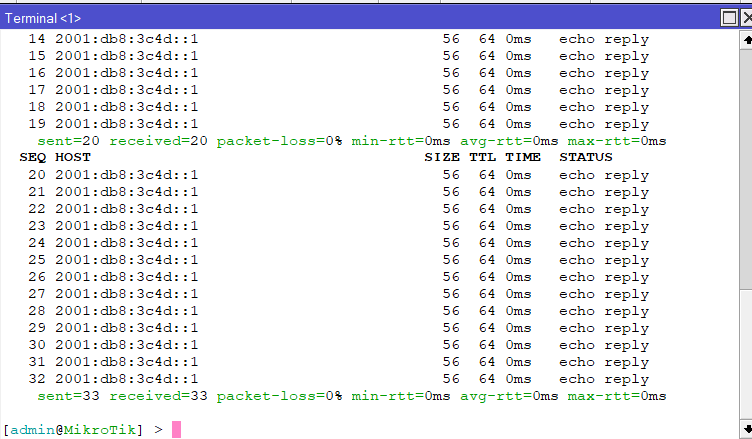
\includegraphics[width=0.7\textwidth]{image/P5/static/static-test.png}    
        
        figure.9 Static v6 Testing
    \end{center}

    \item Dynamic v6 Routing
    
    \begin{center}
        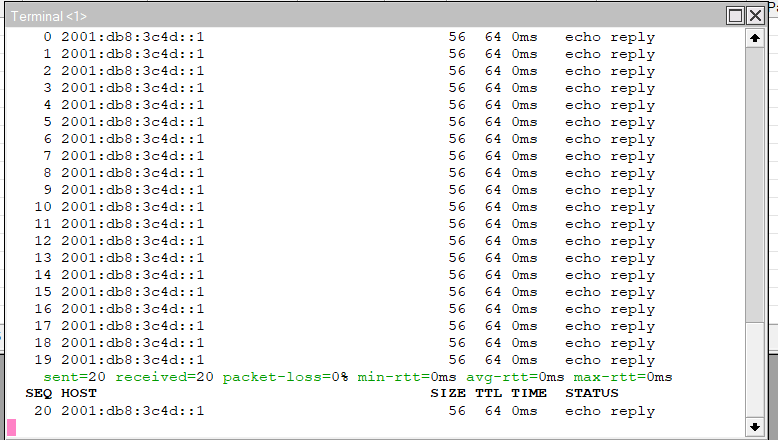
\includegraphics[width=0.7\textwidth]{image/P5/dynamic/dynamic-test.png}    
        
        figure.10 Dynamic v6 Testing
    \end{center}

\end{enumerate}

\section{Kesimpulan}

IPv6 merupakan teknologi baru pengembangan dari IPv4 yang digunakan untuk menigkatkan layanan jaringan internet 

\section{Tugas modul}

\begin{enumerate}
    \item Faktor yang mempengaruhi kinerja koneksi IPv6 antara dua jaringan antara lain:
    \begin{enumerate}
        \item Kualitas dan keandalan perangkat atau infrastruktur jaringan seperti router, switch, dan firewall dapat mempengaruhi kecepatan dan stabilitas koneksi IPv6.
        \item Ketersediaan bandwidth menjadi faktor penting dalam menentukan kinerja koneksi IPv6. Jika bandwidth terbatas, kinerja koneksi IPv6 dapat terpengaruhi dan menyebabkan penurunan kecepatan tranfer data.
        \item Latensi yang tinggi dapat mempengaruhi kinerja koneksi IPv6 dengan menyebabkan penundaan dalam pengiriman data. Beberapa faktor yang dapat menyebabkan latensi tinggi meliputi jarak fisik antara dua jaringan, kualitas jalur jaringan, dan waktu pemrosesan di perangkat jaringan.
        \item Faktor lain yang dapat mempengaruhi kinerja koneksi IPv6 adalah konfigurasi dan pemeliharaan jaringan yang kurang tepat. Kesalahan konfigurasi, kegagalan pemeliharaan rutin, atau kekurangan pembaruan perangkat lunak jaringan dapat mengakibatkan masalah kinerja.
        \item Implementasi kualitas layanan (Quality of Service/QoS).
    \end{enumerate}
    
    \item Untuk menambahkan dua subnet tambahan dengan ukuran /64 dari jaringan IPv6 2001:0db8:1234:://48, dapat dilakukan dengan langkah-langkah berikut:
    
    \begin{enumerate}
        \item Tentukan batas subnet yang diinginkan, karena /64 adalah ukuran defaukt untuk subnet dalam IPv6, maka dapat digunakan dua /64 subnet berurutan dari blok 2001:0db8:1234::/48.
        \item Hitung alamat subnet baru, pertahankan 48 bit pertama dari alamat jaringan 2001:0db8:1234::/48 dan tentukan 16 bit terakhir untuk setiap subnet baru. Ambil 16 bit terakhir dari alamat jaringan, yaitu ::/64 sebagai subnet pertama (alamat subnet pertama 2001:0db8:1234::/64). Tambahkan 1 pada 16 bit terakhir dari alamat subnet pertama, yaitu ::1/64 sebagai subnet kedua (alamat subnet kedua 2001:0db8:1234::1/64).
        \item Setelah menghitung alamat subnet baru, konfigurasi perangkat jaringan yang relevan untuk mengakomodasi subnet tambahan.
        \item Konfigurasikan perangkat klien dengan alamat IPv6 yang tepat dari subnet yang sesuai bila diperlukan.
        
    \end{enumerate}

    Untuk mengkonfigurasi antarmuka jaringan host, dapat dilakukan dengan metode Dynamic Host Configuration Protocol version 6 (DHCPv6) dengan langkan berikut:

    \begin{enumerate}
        \item Pastikan server DHCPv6 terhubung ke subnet baru dan terkonfigurasi dengan benar.
        \item Aktifkan protokol DHCPv6 pada host yang bersangkutan.
        \item Host akan mengirim permintaan alamat IPv6 ke server DHCPv6 dan menerima alamat yang ditugaskan
    \end{enumerate}
    
    \item Migrasi dari IPv4 ke IPv6 diperlukan dalam jaringan saat ini karena beberapa alasan, salah satunya yaitu ketersediaan alamat IPv4 yang semakin menipis. IPv4 menggunakan format alamat 32 bit yang membatasi jumlah alamat yang tersedia, sedangkan IPv6 menggunakan format alamat 128 bit yang dapat memberikan keuntungan kapasitas alamat yang jauh lebih besar dan dapat memenuhi kebutuhan konektivitas di masa depan. Selama proses migrasi, jaringan perlu mendukung koeksistensi IPv4 dan IPv6 untuk memastikan konektivitas yang lancar bagi perangkat yang belum mendukung IPv6. Perlu dipastikan perangkat jaringan dapat melakukan translasi protokol (IPv6-IPv4) dan penyediaan tunel (IPv6-over-IPv4) jika dibutuhkan. Migrasi ke IPv6 membutuhkan perhatian khusus terhadap keamanan jaringan. Perubahan dalam protokol, alamat, dan konfigurasi jaringan dapat mempengaruhi postur keamanan. Penting untuk memastikan bahwa infrastruktur IPv6 terlindungi dengan baik melalui penerapan kebijakan keamanan yang sesuai dan pemantauan lalu lintas jaringan untuk mengidentifikasi dan merespons ancaman keamanan IPv6.
    
\end{enumerate}